\pdfminorversion=4
\documentclass[aspectratio=169]{beamer}

\mode<presentation>
{
  \usetheme{default}
  \usecolortheme{default}
  \usefonttheme{default}
  \setbeamertemplate{navigation symbols}{}
  \setbeamertemplate{caption}[numbered]
  \setbeamertemplate{footline}[frame number]  % or "page number"
  \setbeamercolor{frametitle}{fg=white}
  \setbeamercolor{footline}{fg=black}
}

\usepackage[english]{babel}
\usepackage{inputenc}
\usepackage{tikz}
\usepackage{courier}
\usepackage{array}
\usepackage{bold-extra}
\usepackage{minted}
\usepackage[thicklines]{cancel}
\usepackage{fancyvrb}
\usepackage[normalem]{ulem}

\xdefinecolor{dianablue}{rgb}{0.18,0.24,0.31}
\xdefinecolor{darkblue}{rgb}{0.1,0.1,0.7}
\xdefinecolor{darkgreen}{rgb}{0,0.5,0}
\xdefinecolor{darkgrey}{rgb}{0.35,0.35,0.35}
\xdefinecolor{darkorange}{rgb}{0.8,0.5,0}
\xdefinecolor{darkred}{rgb}{0.7,0,0}
\definecolor{darkgreen}{rgb}{0,0.6,0}
\definecolor{mauve}{rgb}{0.58,0,0.82}

\title[2024-01-10-compute-accelerator-garbage-collectors]{Three garbage collectors: Java, Python, and Julia}
\author{Jim Pivarski}
\institute{Princeton University -- IRIS-HEP}
\date{January 10, 2024}

\usetikzlibrary{shapes.callouts}

\begin{document}

\logo{\pgfputat{\pgfxy(0.11, 7.4)}{\pgfbox[right,base]{\tikz{\filldraw[fill=dianablue, draw=none] (0 cm, 0 cm) rectangle (50 cm, 1 cm);}\mbox{\hspace{-8 cm}
\includegraphics[height=1 cm]{princeton-logo-long.png}\hspace{0.1 cm}\raisebox{0.1 cm}{
\includegraphics[height=0.8 cm]{iris-hep-logo-long.png}}\hspace{0.1 cm}}}}}

\begin{frame}
  \titlepage
\end{frame}

\logo{\pgfputat{\pgfxy(0.11, 7.4)}{\pgfbox[right,base]{\tikz{\filldraw[fill=dianablue, draw=none] (0 cm, 0 cm) rectangle (50 cm, 1 cm);}\mbox{\hspace{-8 cm}
\includegraphics[height=1 cm]{princeton-logo.png}\hspace{0.1 cm}\raisebox{0.1 cm}{
\includegraphics[height=0.8 cm]{iris-hep-logo.png}}\hspace{0.1 cm}}}}}

% Uncomment these lines for an automatically generated outline.
%\begin{frame}{Outline}
%  \tableofcontents
%\end{frame}

% START START START START START START START START START START START START START

\begin{frame}{Dynamic language/programming features}
\vspace{0.2 cm}
\begin{center}
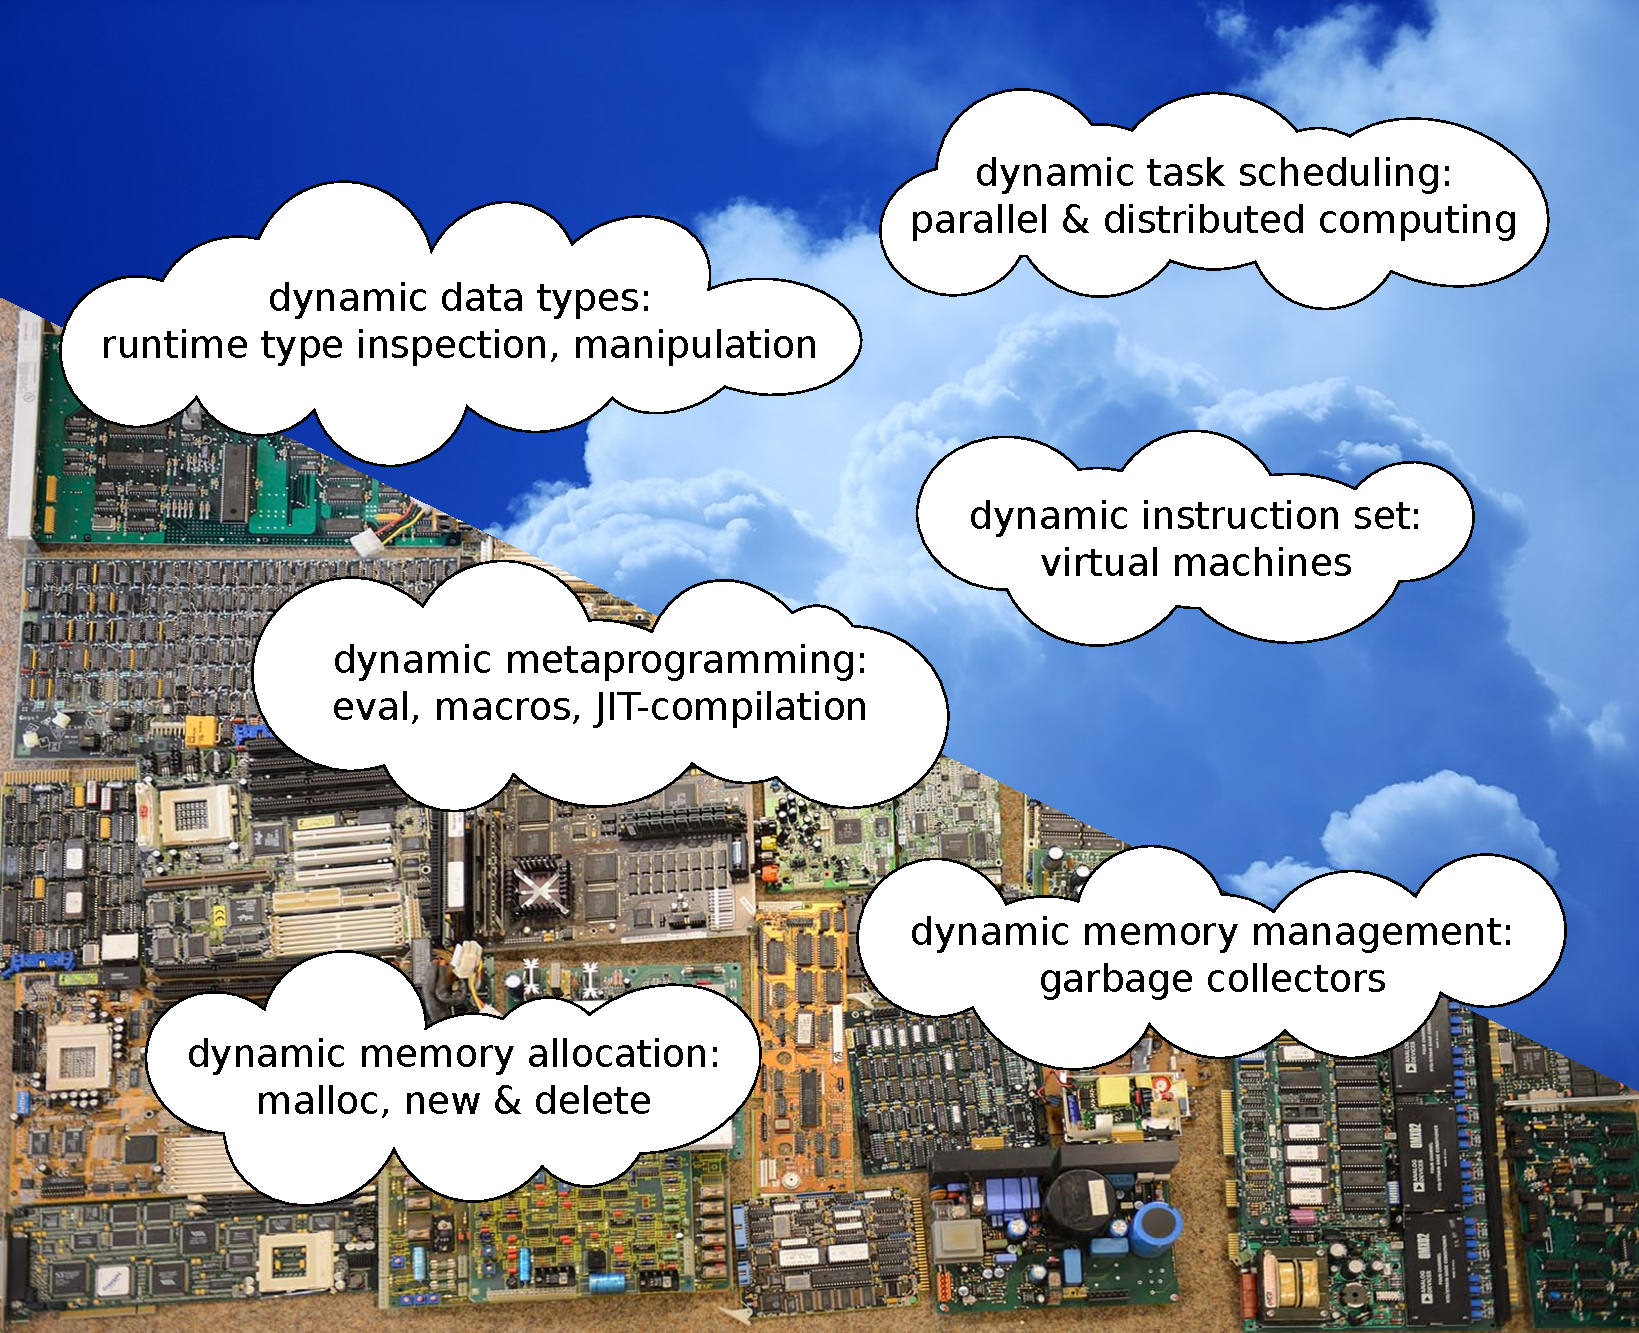
\includegraphics[width=0.67\linewidth]{dynamic-features.pdf}
\end{center}
\end{frame}

\begin{frame}{Dynamic language/programming features}
\begin{columns}
\column{1.15\linewidth}
\begin{center}\renewcommand{\arraystretch}{1.25}
\begin{tabular}{l | c | c | c | c | c | c | c}
                     & alloc   & reference count              & GC      & eval    & VM      & type reflect & scheduling \\\hline
Fortran 77           &          &                                 &         &         &         &         &            \\
C                    & $\surd$  &                                 &         &         &         &         &            \\
C++                  & $\surd$  & {\small\mintinline{c++}{shared_ptr<T>}} &         &         &         & vtable only  & std library \\
C++ with ROOT        & $\surd$  & {\small\mintinline{c++}{shared_ptr<T>}} &         & $\surd$ &         & $\surd$ & $\surd$     \\
Rust                 & $\surd$  & {\small\mintinline{c++}{Rc<T>}}         &         &         &         & vtable only  & $\surd$ \\
Swift                & $\surd$  & $\surd$                         &         &         &         & vtable only  & $\surd$     \\
Julia                & $\surd$  &                                 & $\surd$ & $\surd$ &         & $\surd$ & std macros  \\
Go                   & $\surd$  &                                 & $\surd$ &         &         & vtable only  & $\surd$     \\
Java (JVM languages) & $\surd$  &                                 & $\surd$ &         & $\surd$ & $\surd$ & std library \\
Lua                  & $\surd$  &                                 & $\surd$ & $\surd$ & $\surd$ & $\surd$ &             \\
Python               & $\surd$  & $\surd$                         & $\surd$ & $\surd$ & $\surd$ & $\surd$ & $\surd$     \\
\end{tabular}
\end{center}
\end{columns}
\end{frame}

\begin{frame}{This talk will focus on\ldots}
\begin{columns}[t]
\column{0.001\linewidth}

\column{0.34\linewidth}

\Huge
Java

\vspace{0.5 cm}
\large
Prototypical example of a language with garbage collection; some of our intuitions/preconceptions about garbage collectors are Java-specific.

\column{0.34\linewidth}

\Huge
Python

\vspace{0.5 cm}
\large
Very dynamic language, has both reference counting and mark-and-sweep garbage collection.

\column{0.34\linewidth}

\Huge
Julia

\vspace{0.5 cm}
\large
Up-and-coming language, potentially ideal for HEP. JIT-compiled for bare metal, but has a garbage collector.

\end{columns}
\end{frame}

\begin{frame}{}
\LARGE
\begin{center}
\textcolor{darkblue}{What is the {\it current} status of Julia in HEP?}
\end{center}
\end{frame}

\begin{frame}{State of language use by particle physicists as of last November}
\vspace{0.2 cm}
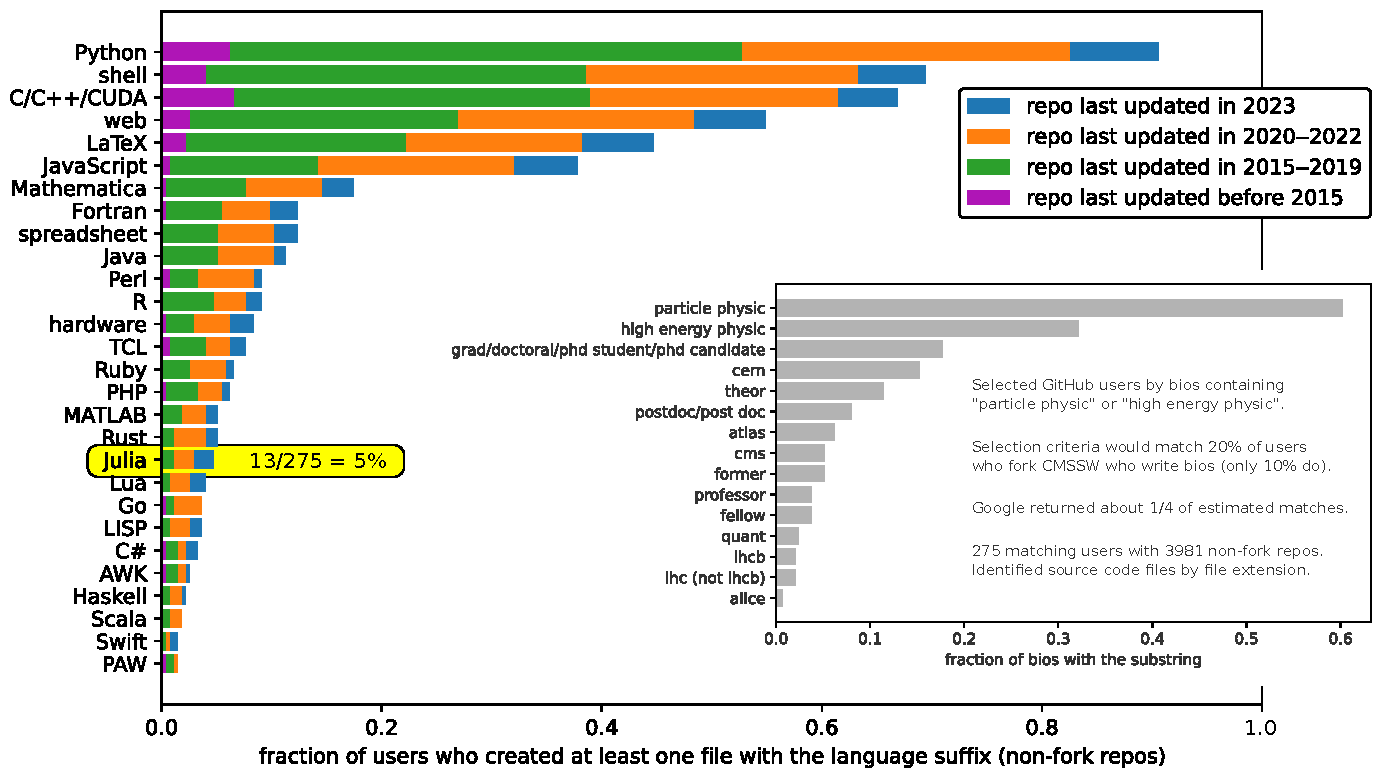
\includegraphics[width=\linewidth]{physicist-languages-presentation.pdf}
\end{frame}

\begin{frame}{But physicists are more interested in Julia than, say, Rust or Lua}
\vspace{0.5 cm}
Among ``Materials'' (PDFs and TXTs) in CERN's Indico search since January 2022,

\vspace{0.25 cm}
\begin{description}
\item[\textcolor{darkorange}{\bf 63}] \textcolor{darkorange}{\bf refer to Julia the programming language}
\item[324] refer to people named Julia
\item[4] other/unclear
\end{description}

\begin{description}
\item[\textcolor{darkorange}{\bf 12}] \textcolor{darkorange}{\bf refer to Rust the programming language}

(7 of those same documents also refer to Julia)
\item[10] refer to oxidized metal
\item[3] other/unclear
\end{description}

\begin{description}
\item[\textcolor{darkorange}{\bf 1}] \textcolor{darkorange}{\bf refers to Lua the programming language}

(it's used to configure the SIMION charged particle simulator)
\item[4] refer to the LHC User's Association
\item[4] other/unclear
\end{description}
\end{frame}

\begin{frame}{Similarly, Julia is increasingly a focus on ACAT and CHEP}
\vspace{0.5 cm}

\textcolor{darkblue}{\Large\bf ACAT 2022:}
\begin{itemize}
\item Julia: 1 title and 1 abstract
\item Python: 3 titles and 24 abstracts
\end{itemize}

\vspace{0.5 cm}
\textcolor{darkblue}{\Large\bf CHEP 2023:}
\begin{itemize}
\item Julia: 3 titles and 4 abstracts
\item Python: 1 title and 35 abstracts
\end{itemize}

\vspace{0.5 cm}
Only other programming languages mentioned: C++ (frequently) and Java (2 times).
\end{frame}

\begin{frame}{Julia has an HSF working group, meetings, and annual workshops}
\vspace{0.05 cm}
\begin{center}

\includegraphics[width=0.72\linewidth]{juliahep-website.png}
\end{center}
\end{frame}

\begin{frame}{}
\LARGE
\begin{center}
\textcolor{darkblue}{Back to garbage collectors}
\end{center}
\end{frame}

\begin{frame}[fragile]{Reference counting}
\vspace{0.4 cm}
\small

\begin{minted}{python}
>>> import sys
\end{minted}
\vspace{0.1 cm}
\small
\begin{minted}{python}
>>> x = object()
>>> sys.getrefcount(x)
2
\end{minted}

\begin{uncoverenv}<2->
\vspace{0.1 cm}
\begin{minted}{python}
>>> y = x
>>> sys.getrefcount(x)
3
\end{minted}
\end{uncoverenv}

\begin{uncoverenv}<3->
\vspace{0.1 cm}
\begin{minted}{python}
>>> z = [x, x, x, x, x]
>>> sys.getrefcount(x)
8
\end{minted}
\end{uncoverenv}

\begin{uncoverenv}<4->
\vspace{0.1 cm}
\begin{minted}{python}
>>> del x, z
>>> sys.getrefcount(y)
2
\end{minted}
\end{uncoverenv}

\begin{uncoverenv}<5->
\vspace{-5 cm}
\hfill 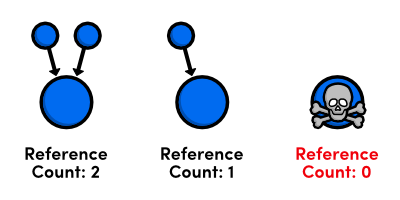
\includegraphics[width=6 cm]{reference-counting.png} \hspace{0.75 cm}
\vspace{5 cm}
\end{uncoverenv}
\end{frame}

\begin{frame}[fragile]{The problem with reference counting}
\vspace{0.4 cm}
\small
\begin{minted}{python}
>>> class HasDestructor:
...     def __del__(self):
...         print("Goodbye, world")
... 
\end{minted}
\vspace{0.1 cm}
\begin{minted}{python}
>>> x = HasDestructor()
>>> del x
Goodbye, world
\end{minted}

\begin{uncoverenv}<2->
\vspace{0.1 cm}
\begin{minted}{python}
>>> y = HasDestructor()
>>> y.self = y
>>> del y
\end{minted}
\end{uncoverenv}

\begin{uncoverenv}<4->
\vspace{0.1 cm}
\begin{minted}{python}
>>> import gc
>>> gc.collect()
Goodbye, world
47
\end{minted}
\end{uncoverenv}

\begin{uncoverenv}<3->
\vspace{-3.5 cm}
\hfill \begin{minipage}{7.75 cm} All references to \mintinline{python}{y} are gone: it can't be accessed anymore. But it has not been deleted (\mintinline{python}{__del__} has not been called) because its self-reference keeps its reference count from reaching zero.\end{minipage}
\vspace{3.5 cm}
\end{uncoverenv}

\begin{uncoverenv}<5->
\vspace{-2.7 cm}
\hfill \begin{minipage}{7.75 cm} Now it's gone.\end{minipage}
\vspace{2.7 cm}
\end{uncoverenv}
\end{frame}

\begin{frame}{A common garbage collection algorithm}
\vspace{0.5 cm}
\only<1>{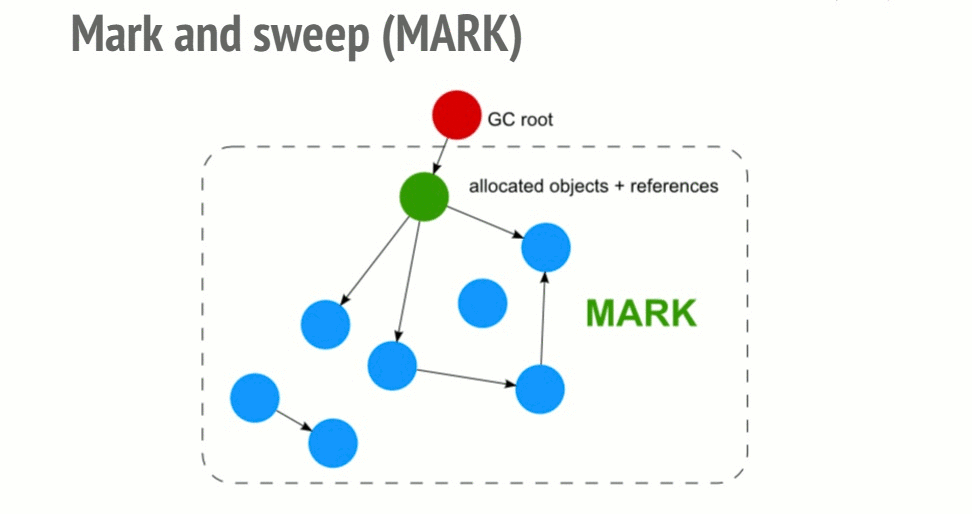
\includegraphics[width=\linewidth]{mark-and-sweep-1.png}}\only<2>{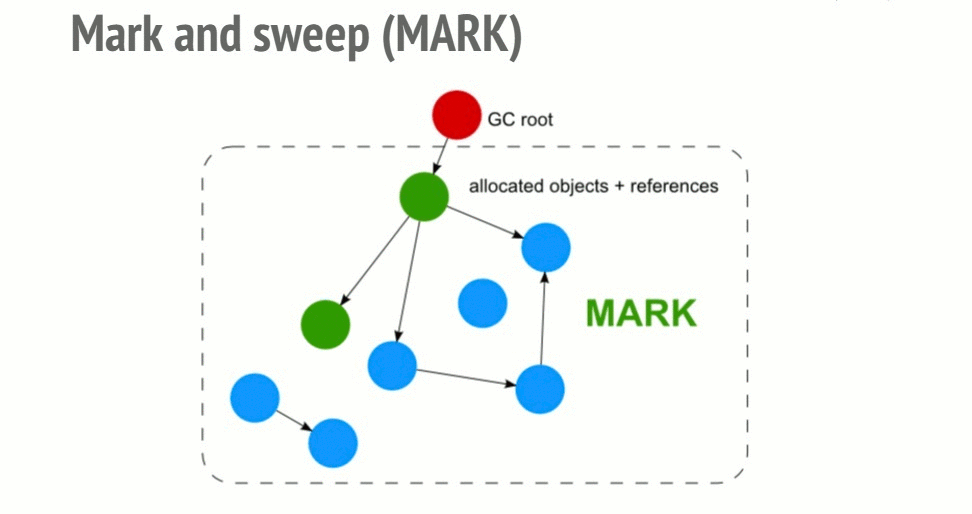
\includegraphics[width=\linewidth]{mark-and-sweep-2.png}}\only<3>{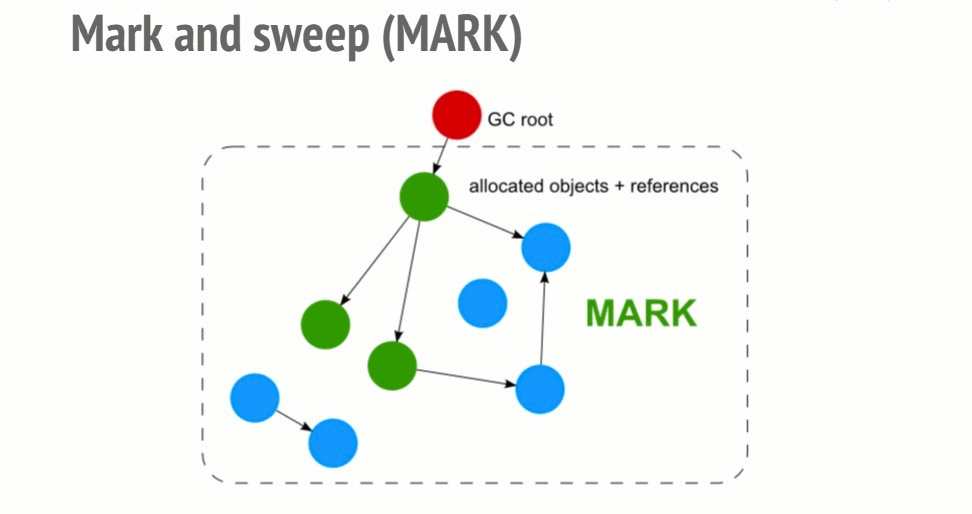
\includegraphics[width=\linewidth]{mark-and-sweep-3.png}}\only<4>{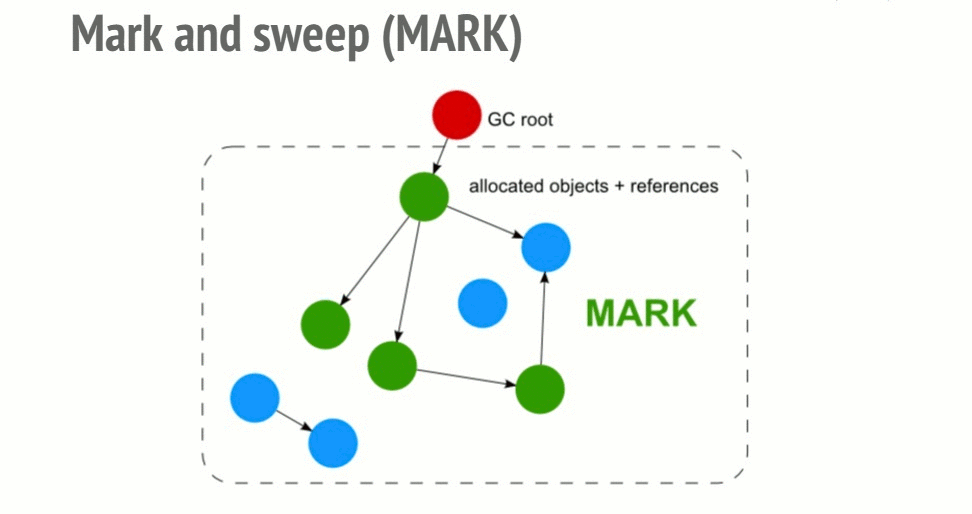
\includegraphics[width=\linewidth]{mark-and-sweep-4.png}}\only<5>{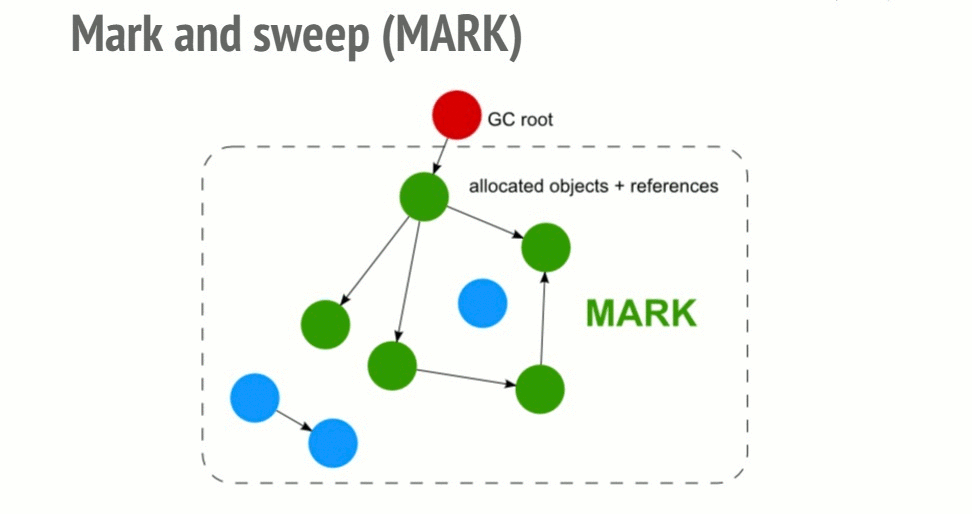
\includegraphics[width=\linewidth]{mark-and-sweep-5.png}}\only<6>{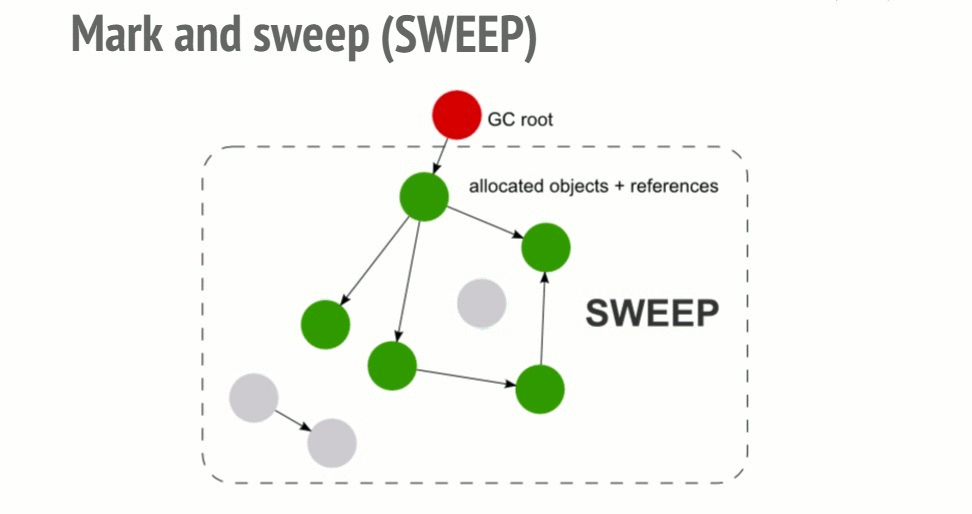
\includegraphics[width=\linewidth]{mark-and-sweep-6.png}}\only<7>{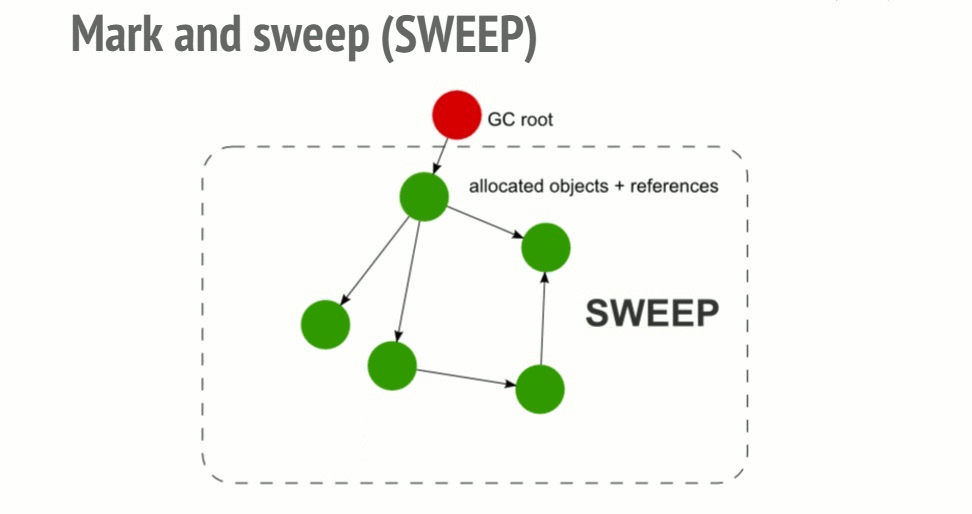
\includegraphics[width=\linewidth]{mark-and-sweep-7.png}}
\end{frame}

\begin{frame}{Garbage collector generations}
\begin{center}
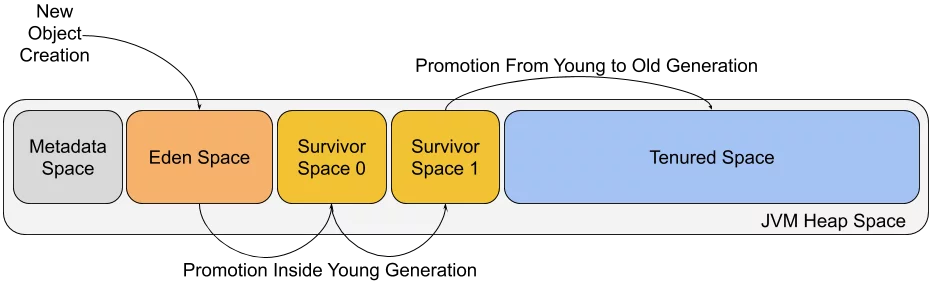
\includegraphics[width=\linewidth]{java-collection-6.png}
\end{center}
\end{frame}

\begin{frame}[fragile]{Example in Python, which has 3 generations}
\small
\begin{columns}
\column{1.09\linewidth}
\begin{minted}{python}
>>> import gc
>>> _ = gc.collect(); gc.disable()
>>> [len(gc.get_objects(gen)) for gen in (0, 1, 2)]
[8, 0, 8220]
\end{minted}

\begin{uncoverenv}<2->
\begin{minted}{python}
>>> import uproot
>>> [len(gc.get_objects(gen)) for gen in (0, 1, 2)]
[57034, 0, 8199]
\end{minted}
\end{uncoverenv}

\begin{uncoverenv}<3->
\begin{minted}{python}
>>> _ = gc.collect(); [len(gc.get_objects(gen)) for gen in (0, 1, 2)]
[3, 0, 39192]
\end{minted}
\end{uncoverenv}

\begin{uncoverenv}<4->
\begin{minted}{python}
>>> uproot.open("Zmumu.root:events").arrays()
<Array [{Type: 'GT', Run: 148031, ...}, ...] type='2304 * {Type: stri...'>
>>> [len(gc.get_objects(gen)) for gen in (0, 1, 2)]
[33573, 0, 39136]
\end{minted}
\end{uncoverenv}

\begin{uncoverenv}<5->
\begin{minted}{python}
>>> _ = gc.collect(); [len(gc.get_objects(gen)) for gen in (0, 1, 2)]
[3, 0, 56692]
\end{minted}
\end{uncoverenv}
\end{columns}
\end{frame}

\begin{frame}{Differences among the three languages}
\vspace{0.1 cm}
\Huge
Java \hfill {\tiny \begin{minipage}{0.8\linewidth}\hfill \textcolor{blue}{\url{https://www.oracle.com/webfolder/technetwork/tutorials/obe/java/gc01/index.html}}

\hfill \textcolor{blue}{\url{https://abiasforaction.net/category/java/gc}}\end{minipage}}

\vspace{0.25 cm}
\normalsize
Rather than calling \mintinline{c}{malloc} for each new object, objects are made from preallocated memory pools. Each pool represents a different generation; those that survive mark-and-sweep are {\it copied} from one pool into the next.

\begin{center}
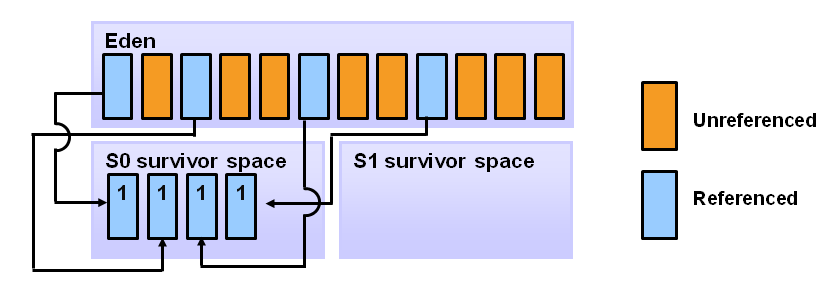
\includegraphics[width=0.7\linewidth]{java-generations-compactifications.png}
\end{center}

No stable pointers, but it keeps the memory unfragmented: finding space for new objects is fast (i.e.\ especially good for making many short-lived objects).
\end{frame}

\begin{frame}[fragile]{Differences among the three languages}
\vspace{0.1 cm}
\Huge
Python \hfill {\tiny \begin{minipage}{0.7\linewidth}\hfill \textcolor{blue}{\url{https://devguide.python.org/internals/garbage-collector}}

\hfill \textcolor{blue}{\url{https://docs.python.org/3/c-api/memory.html}}

\hfill \textcolor{blue}{\url{https://docs.python.org/3/using/cmdline.html\#envvar-PYTHONMALLOC}}\end{minipage}}

\vspace{0.25 cm}
\normalsize
CPython relies on reference counting for most memory management; full garbage collection is just to clean up cycles. (PyPy only has full garbage collection.)

\vspace{0.2 cm}
The 3 generations are different doubly-linked lists. Mark-and-sweep marks are in the low bits of the list pointers so that garbage collection has a constant memory footprint.

\tiny
\begin{verbatim}
                           +--+--+--+--+--+--+--+--+--+--+--+--+--+--+--+--+ \
                           |                    *_gc_next                  | |
                           +--+--+--+--+--+--+--+--+--+--+--+--+--+--+--+--+ | PyGC_Head
                           |                    *_gc_prev                  | |
             object -----> +--+--+--+--+--+--+--+--+--+--+--+--+--+--+--+--+ /
                           |                    ob_refcnt                  | \
                           +--+--+--+--+--+--+--+--+--+--+--+--+--+--+--+--+ | PyObject_HEAD
                           |                    *ob_type                   | |
                           +--+--+--+--+--+--+--+--+--+--+--+--+--+--+--+--+ /
                           |                      ...                      |
\end{verbatim}

\normalsize
Objects have stable pointers, which are good for C/C++ extensions, but not managed by \mintinline{c}{malloc} (depends on \mintinline{bash}{PYTHONMALLOC} environment variable and Python build).
\end{frame}

\begin{frame}[fragile]{Differences among the three languages}
\vspace{0.1 cm}
\Huge
Julia \hfill {\tiny \begin{minipage}{0.8\linewidth}\hfill \textcolor{blue}{\url{https://docs.julialang.org/en/v1/devdocs/gc}}

\hfill \textcolor{blue}{\url{https://discourse.julialang.org/t/18021/3}}

\hfill \textcolor{blue}{\url{https://docs.julialang.org/en/v1/devdocs/object}}

\hfill \textcolor{blue}{\url{https://github.com/JuliaLang/julia/blob/v1.10.0/src/julia.h\#L106-L114}}\end{minipage}}

\vspace{0.25 cm}
\normalsize
$< 2$~kB objects are managed in pools, allocated by page; large objects use \mintinline{c}{malloc}.

\vspace{0.2 cm}
Objects have headers for type reflection, and the first 2 bits are a mark-and-sweep mark and a generation (1 bit = 2 generations).

\small
\begin{minted}{c}
      typedef struct {
          opaque metadata;    /* sizeof(uintptr_t) header */
          jl_value_t value;   /* actual data */
      } jl_taggedvalue_t;
\end{minted}

\vspace{0.2 cm}
\normalsize
Marking is depth-first and parallel; sweeping is serial. Memory is returned to the operating system on a per-page basis. Once a page has zero surviving objects, it is freed using \mintinline{c}{madvise} on a background thread.

\vspace{0.2 cm}
Julia makes stack-versus-heap user-visible, to help users avoid garbage collection.
\end{frame}

\begin{frame}{}
\LARGE
\begin{center}
\textcolor{darkblue}{Experiments on garbage collectors}
\end{center}
\end{frame}

\begin{frame}[fragile]{Replacing objects with a lifespan of $16 \pm 0$ steps}
\small
\begin{columns}
\column{1.07\linewidth}
\begin{minted}{python}
shuffleA = [7, 6, 4, 10, 0, 15, 9, 8, 13, 5, 12, 14, 3, 11, 2, 1]
shuffleB = [3, 8, 0, 15, 11, 2, 6, 7, 12, 9, 1, 14, 5, 13, 4, 10]
shuffleC = [2, 13, 6, 7, 4, 5, 10, 3, 12, 15, 8, 9, 14, 1, 0, 11]
shuffleD = [7, 5, 9, 15, 4, 2, 13, 12, 0, 8, 11, 6, 3, 1, 10, 14]
shuffleE = [14, 11, 10, 8, 0, 6, 5, 1, 13, 9, 7, 4, 2, 12, 3, 15]
array = np.empty(16**5, dtype=object)
for iA in shuffleA:
  for iB in shuffleB:
    for iC in shuffleC:
      for iD in shuffleD:
        for iE in shuffleE:
          array[(((iA*16 + iB)*16 + iC)*16 + iD)*16 + iE] = []




        for iE in shuffleE:
          array[(((iA*16 + iB)*16 + iC)*16 + iD)*16 + iE] = []
\end{minted}
\end{columns}
\end{frame}

\begin{frame}[fragile]{Replacing objects with a lifespan of $16^2 = 256 \pm 0$ steps}
\small
\begin{columns}
\column{1.07\linewidth}
\begin{minted}{python}
shuffleA = [7, 6, 4, 10, 0, 15, 9, 8, 13, 5, 12, 14, 3, 11, 2, 1]
shuffleB = [3, 8, 0, 15, 11, 2, 6, 7, 12, 9, 1, 14, 5, 13, 4, 10]
shuffleC = [2, 13, 6, 7, 4, 5, 10, 3, 12, 15, 8, 9, 14, 1, 0, 11]
shuffleD = [7, 5, 9, 15, 4, 2, 13, 12, 0, 8, 11, 6, 3, 1, 10, 14]
shuffleE = [14, 11, 10, 8, 0, 6, 5, 1, 13, 9, 7, 4, 2, 12, 3, 15]
array = np.empty(16**5, dtype=object)
for iA in shuffleA:
  for iB in shuffleB:
    for iC in shuffleC:
      for iD in shuffleD:
        for iE in shuffleE:
          array[(((iA*16 + iB)*16 + iC)*16 + iD)*16 + iE] = []



      for iD in shuffleD:
        for iE in shuffleE:
          array[(((iA*16 + iB)*16 + iC)*16 + iD)*16 + iE] = []
\end{minted}
\end{columns}
\end{frame}

\begin{frame}[fragile]{Replacing objects with a lifespan of $16^3 = 4096 \pm 0$ steps}
\small
\begin{columns}
\column{1.07\linewidth}
\begin{minted}{python}
shuffleA = [7, 6, 4, 10, 0, 15, 9, 8, 13, 5, 12, 14, 3, 11, 2, 1]
shuffleB = [3, 8, 0, 15, 11, 2, 6, 7, 12, 9, 1, 14, 5, 13, 4, 10]
shuffleC = [2, 13, 6, 7, 4, 5, 10, 3, 12, 15, 8, 9, 14, 1, 0, 11]
shuffleD = [7, 5, 9, 15, 4, 2, 13, 12, 0, 8, 11, 6, 3, 1, 10, 14]
shuffleE = [14, 11, 10, 8, 0, 6, 5, 1, 13, 9, 7, 4, 2, 12, 3, 15]
array = np.empty(16**5, dtype=object)
for iA in shuffleA:
  for iB in shuffleB:
    for iC in shuffleC:
      for iD in shuffleD:
        for iE in shuffleE:
          array[(((iA*16 + iB)*16 + iC)*16 + iD)*16 + iE] = []


    for iC in shuffleC:
      for iD in shuffleD:
        for iE in shuffleE:
          array[(((iA*16 + iB)*16 + iC)*16 + iD)*16 + iE] = []
\end{minted}
\end{columns}
\end{frame}

\begin{frame}[fragile]{Replacing objects with a lifespan of $16^4 = 65536 \pm 0$ steps}
\small
\begin{columns}
\column{1.07\linewidth}
\begin{minted}{python}
shuffleA = [7, 6, 4, 10, 0, 15, 9, 8, 13, 5, 12, 14, 3, 11, 2, 1]
shuffleB = [3, 8, 0, 15, 11, 2, 6, 7, 12, 9, 1, 14, 5, 13, 4, 10]
shuffleC = [2, 13, 6, 7, 4, 5, 10, 3, 12, 15, 8, 9, 14, 1, 0, 11]
shuffleD = [7, 5, 9, 15, 4, 2, 13, 12, 0, 8, 11, 6, 3, 1, 10, 14]
shuffleE = [14, 11, 10, 8, 0, 6, 5, 1, 13, 9, 7, 4, 2, 12, 3, 15]
array = np.empty(16**5, dtype=object)
for iA in shuffleA:
  for iB in shuffleB:
    for iC in shuffleC:
      for iD in shuffleD:
        for iE in shuffleE:
          array[(((iA*16 + iB)*16 + iC)*16 + iD)*16 + iE] = []

  for iB in shuffleB:
    for iC in shuffleC:
      for iD in shuffleD:
        for iE in shuffleE:
          array[(((iA*16 + iB)*16 + iC)*16 + iD)*16 + iE] = []
\end{minted}
\end{columns}
\end{frame}

\begin{frame}[fragile]{Replacing objects with a lifespan of $16^5 = 1048576 \pm 0$ steps}
\small
\begin{columns}
\column{1.07\linewidth}
\begin{minted}{python}
shuffleA = [7, 6, 4, 10, 0, 15, 9, 8, 13, 5, 12, 14, 3, 11, 2, 1]
shuffleB = [3, 8, 0, 15, 11, 2, 6, 7, 12, 9, 1, 14, 5, 13, 4, 10]
shuffleC = [2, 13, 6, 7, 4, 5, 10, 3, 12, 15, 8, 9, 14, 1, 0, 11]
shuffleD = [7, 5, 9, 15, 4, 2, 13, 12, 0, 8, 11, 6, 3, 1, 10, 14]
shuffleE = [14, 11, 10, 8, 0, 6, 5, 1, 13, 9, 7, 4, 2, 12, 3, 15]
array = np.empty(16**5, dtype=object)
for iA in shuffleA:
  for iB in shuffleB:
    for iC in shuffleC:
      for iD in shuffleD:
        for iE in shuffleE:
          array[(((iA*16 + iB)*16 + iC)*16 + iD)*16 + iE] = []
for iA in shuffleA:
  for iB in shuffleB:
    for iC in shuffleC:
      for iD in shuffleD:
        for iE in shuffleE:
          array[(((iA*16 + iB)*16 + iC)*16 + iD)*16 + iE] = []
\end{minted}
\end{columns}
\end{frame}

\begin{frame}[fragile]{Replacing objects with a lifespan of $16^2 = 256 \pm 97.8$ steps}
\small
\begin{columns}
\column{1.07\linewidth}
\begin{minted}{python}
shuffleA = [7, 6, 4, 10, 0, 15, 9, 8, 13, 5, 12, 14, 3, 11, 2, 1]
shuffleB = [3, 8, 0, 15, 11, 2, 6, 7, 12, 9, 1, 14, 5, 13, 4, 10]
shuffleC = [2, 13, 6, 7, 4, 5, 10, 3, 12, 15, 8, 9, 14, 1, 0, 11]
shuffleD = [7, 5, 9, 15, 4, 2, 13, 12, 0, 8, 11, 6, 3, 1, 10, 14]
shuffleE = [14, 11, 10, 8, 0, 6, 5, 1, 13, 9, 7, 4, 2, 12, 3, 15]
array = np.empty(16**5, dtype=object)
for iA in shuffleA:
  for iB in shuffleB:
    for iC in shuffleC:
      for iD in shuffleD:
        for iE in shuffleE:
          array[(((iA*16 + iB)*16 + iC)*16 + iD)*16 + iE] = []



      for iE in shuffleE:
        for iD in shuffleD:
          array[(((iA*16 + iB)*16 + iC)*16 + iD)*16 + iE] = []
\end{minted}
\end{columns}
\end{frame}

\begin{frame}[fragile]{Replacing objects with a lifespan of $16^3 = 4096 \pm 1660$ steps}
\small
\begin{columns}
\column{1.07\linewidth}
\begin{minted}{python}
shuffleA = [7, 6, 4, 10, 0, 15, 9, 8, 13, 5, 12, 14, 3, 11, 2, 1]
shuffleB = [3, 8, 0, 15, 11, 2, 6, 7, 12, 9, 1, 14, 5, 13, 4, 10]
shuffleC = [2, 13, 6, 7, 4, 5, 10, 3, 12, 15, 8, 9, 14, 1, 0, 11]
shuffleD = [7, 5, 9, 15, 4, 2, 13, 12, 0, 8, 11, 6, 3, 1, 10, 14]
shuffleE = [14, 11, 10, 8, 0, 6, 5, 1, 13, 9, 7, 4, 2, 12, 3, 15]
array = np.empty(16**5, dtype=object)
for iA in shuffleA:
  for iB in shuffleB:
    for iC in shuffleC:
      for iD in shuffleD:
        for iE in shuffleE:
          array[(((iA*16 + iB)*16 + iC)*16 + iD)*16 + iE] = []


    for iE in shuffleE:
      for iD in shuffleD:
        for iC in shuffleC:
          array[(((iA*16 + iB)*16 + iC)*16 + iD)*16 + iE] = []
\end{minted}
\end{columns}
\end{frame}

\begin{frame}[fragile]{Replacing objects with a lifespan of $16^4 = 65\,536 \pm 26\,700$ steps}
\small
\begin{columns}
\column{1.07\linewidth}
\begin{minted}{python}
shuffleA = [7, 6, 4, 10, 0, 15, 9, 8, 13, 5, 12, 14, 3, 11, 2, 1]
shuffleB = [3, 8, 0, 15, 11, 2, 6, 7, 12, 9, 1, 14, 5, 13, 4, 10]
shuffleC = [2, 13, 6, 7, 4, 5, 10, 3, 12, 15, 8, 9, 14, 1, 0, 11]
shuffleD = [7, 5, 9, 15, 4, 2, 13, 12, 0, 8, 11, 6, 3, 1, 10, 14]
shuffleE = [14, 11, 10, 8, 0, 6, 5, 1, 13, 9, 7, 4, 2, 12, 3, 15]
array = np.empty(16**5, dtype=object)
for iA in shuffleA:
  for iB in shuffleB:
    for iC in shuffleC:
      for iD in shuffleD:
        for iE in shuffleE:
          array[(((iA*16 + iB)*16 + iC)*16 + iD)*16 + iE] = []

  for iE in shuffleE:
    for iD in shuffleD:
      for iC in shuffleC:
        for iB in shuffleB:
          array[(((iA*16 + iB)*16 + iC)*16 + iD)*16 + iE] = []
\end{minted}
\end{columns}
\end{frame}

\begin{frame}[fragile]{Replacing objects with a lifespan of $16^5 = 1\,048\,576 \pm 428\,000$ steps}
\small
\begin{columns}
\column{1.07\linewidth}
\begin{minted}{python}
shuffleA = [7, 6, 4, 10, 0, 15, 9, 8, 13, 5, 12, 14, 3, 11, 2, 1]
shuffleB = [3, 8, 0, 15, 11, 2, 6, 7, 12, 9, 1, 14, 5, 13, 4, 10]
shuffleC = [2, 13, 6, 7, 4, 5, 10, 3, 12, 15, 8, 9, 14, 1, 0, 11]
shuffleD = [7, 5, 9, 15, 4, 2, 13, 12, 0, 8, 11, 6, 3, 1, 10, 14]
shuffleE = [14, 11, 10, 8, 0, 6, 5, 1, 13, 9, 7, 4, 2, 12, 3, 15]
array = np.empty(16**5, dtype=object)
for iA in shuffleA:
  for iB in shuffleB:
    for iC in shuffleC:
      for iD in shuffleD:
        for iE in shuffleE:
          array[(((iA*16 + iB)*16 + iC)*16 + iD)*16 + iE] = []
for iE in shuffleE:
  for iD in shuffleD:
    for iC in shuffleC:
      for iB in shuffleB:
        for iA in shuffleA:
          array[(((iA*16 + iB)*16 + iC)*16 + iD)*16 + iE] = []
\end{minted}
\end{columns}
\end{frame}

\begin{frame}[fragile]{Replacing objects in Julia}
\small
\begin{columns}
\column{1.07\linewidth}
\begin{minted}{julia}
shuffleA::Vector{Int64} = [ 7,  6,  4, 10,  0, 15,  9,  8,
                           13,  5, 12, 14,  3, 11,  2,  1]
...
array::Vector{Union{Vector{Int32},Nothing}} = fill(nothing, 16^5)
for iA in shuffleA
  for iB in shuffleB
    for iC in shuffleC
      for iD in shuffleD
        for iE in shuffleE
          array[(((iA*16 + iB)*16 + iC)*16 + iD)*16 + iE + 1] = []
        end
        for iE in shuffleE
          array[(((iA*16 + iB)*16 + iC)*16 + iD)*16 + iE + 1] = []
        end
      end
    end
  end
end
\end{minted}
\end{columns}
\end{frame}

\begin{frame}[fragile]{Replacing objects on the JVM (Scala)}
\small
\begin{columns}
\column{1.07\linewidth}
\begin{minted}{scala}
val shuffleA = Array[Int]( 7,  6,  4, 10,  0, 15,  9,  8,
                          13,  5, 12, 14,  3, 11,  2,  1)
...
val array = Array.fill(Math.pow(16, 5).toInt)(Option.empty[Array[Int]])
for (iA <- shuffleA) {
  for (iB <- shuffleB) {
    for (iC <- shuffleC) {
      for (iD <- shuffleD) {
        for (iE <- shuffleE)
          array(((((iA*16 + iB)*16 + iC)*16 + iD)*16 + iE)) =
              Some(Array[Int]())
        for (iE <- shuffleE)
          array(((((iA*16 + iB)*16 + iC)*16 + iD)*16 + iE)) =
              Some(Array[Int]())
      }
    }
  }
}
\end{minted}
\end{columns}
\end{frame}

\begin{frame}[fragile]{Measuring time uniformly across languages}
\vspace{0.3 cm}
The Scala, Python, and Julia processes each send a byte (\mintinline{python}{'.'}) to a separate C++ process every 2048 ($2^{11}$) steps, which is listening to an unbuffered, localhost socket.

\vspace{0.2 cm}
The C++ process records time differences between each received byte.

\small
\vspace{0.3 cm}
\begin{minted}{c++}
using std::chrono;

do {
  recv(new_socket, buffer, 1, 0);
  stop = std::chrono::steady_clock::now();
  printf("%d\n", duration_cast<microseconds>(stop - start).count());
  start = stop;
}
while (buffer[0] == '.');
\end{minted}

\normalsize
\vspace{0.3 cm}
When Scala, Python, or Julia encounter a garbage collector pause, it shows up as an unusually long time between pings.
\end{frame}

\end{document}

%% Yes, I've run into performance problems with garbage collectors in previous projects, though they were particular situations that can perhaps be avoided.

%% Specifically, I was working in Java, developing a distributed pipeline. When one step passed data along to another step, it would go into the latter's input queue. The problem was that this JVM would occasionally pause for garbage collection, and during that time, its input queue filled up. With a lot more (garbage collectable) objects in the input queue, it would have more garbage collection to do, and the situation spiraled out of control—it was a positive feedback loop. It was too late to re-architect the whole workflow, so I switched Java's default garbage collector for a pauseless one and tuned it until we had a working system if it stayed within certain parameters.

%% That's a more specific problem than just having long-running jobs. I can't think of any particular issue with long-running jobs and garbage collectors—it's not unusual for Python processes to be long-running.

%% Another issue with garbage collectors (more recent Python experience) is that they make memory performance harder to debug. Often, Uproot users report memory leaks when they see memory use increase linearly in a loop, but then when I investigate, it turns out that the garbage collector just hadn't decided to trigger yet. When it does, the memory use becomes flat. (This isn't always the case: users have reported real, significant memory leaks. It's just harder to debug because sometimes it's a mismatch between their assumption that the memory will be released immediately when in fact the collector just hasn't triggered yet.)

%% On this point, an important question is, "what triggers garbage collection?" That's something I've been intending to understand better. I had previously thought that Linux processes knew how much memory is available and would trigger garbage collection when, say, they've reached the 90% limit. I've done some experiments putting processes in a memory-limited box like

%% systemd-run --user --scope -p MemoryMax=100M -p MemorySwapMax=0M python ...

%% and I see that they trigger garbage collection earlier, to stay within the box. But Enrico Guiraud told me that Linux has no such mechanism, so I'm going to need to do some reading and more experiments to be sure.

%% Summary of three garbage collectors:
%% Java:
%% compactifies (copies) data in generational buckets, so all references are pointers-to-pointers (pointer chasing)
%% many options, and the default has changed through the years
%% old default would "stop the world," which was my problem with the distributed workflow; new default from Java 15 onward is pauseless
%% Python:
%% reference counting is the primary collector (in CPython, not PyPy), so data without reference cycles should get freed immediately after going out of scope; reference counters use a lot of memory, though
%% uses a number of allocations (in three generations) since last collection to decide when to trigger (reference, I just found this), then it's a stop-the-world mark-and-sweep
%% allocates data into its own arenas, so the memory use reported to the operating system can be more than what Python is actually using; that could explain some of the spurious memory leak reports
%% Julia:
%% summary from the documentation; summary from Stefan Karpinsk
%% no compactification and no reference counters: all garbage collector information is encoded in two bits of tagged pointers, one for the mark-and-sweep mark, and another for age (so exactly two generations, then)
%% Julia's pool allocation of small objects sounds to me like the private arenas that complicate Python memory debugging, but the same page says that it malloc's arrays and large objects, so it might not matter (you only need to debug large memory issues)
%% this comment from Sep 2021 leads me to believe that Julia's garbage collector is single-threaded and stops the world: "That’s basically how I can see the GC pauses: when the computation only eats 1 CPU as seen in htop." This StackOverflow answer would confirm it, but it's 8 years old. Do you have more recent information on these two aspects of Julia's garbage collector, is it multithreaded and does it pause execution?
%% I also don't know if it's possible to tune Julia's garbage collector nowadays
%% instead of exclusively relying on the garbage collector, as Java and Python mostly* do, Julia tries to get as many objects as possible on the stack, rather than the heap. Immutable data structures are preferred in order to encourage this (tutorial, HackerNews). I had thought there was a way to force Julia objects onto the stack with a macro, but I couldn't find it on the Performance Hints page. Anyway, stack allocation (and performance in general) is a more frequent topic of discussion in Julia circles than in Java and Python.
%% * Java and Python have internal optimizations to use the stack when escape analysis says it's possible, but less aggressively than Julia.

%% So, just being a long-running process doesn't sound to me like a reason to avoid garbage collectors, but I don't know the rest of the context. In fact, the memory safety that garbage collectors (or Rust) provide sounds important for a long-running process: the probability of mistakes in manual memory management is compounded by time.

%% I had particular issues with a stop-the-world garbage collector in the past, but that situation can be avoided with workflow design, once you know that it can be an issue.

%% Finally, a language is not just the technical details of its implementation; it's also a community that has certain priorities. The Julia community is obsessed with performance, so it's easy to get help about performance issues (and hard to avoid getting performance hints when your question is not performance related...). If it's really true that the Julia garbage collector is still single-threaded, stop-the-world, I'd be surprised, but there would also be a lot of motivation in the community to fix it or at least point out ways to avoid heap-allocation.
